\documentclass{article}
\usepackage[utf8]{inputenc}
\usepackage{amsmath}
\usepackage{tcolorbox}
\usepackage[margin=1in]{geometry}
\usepackage{listings}
\usepackage{xcolor}

\definecolor{codegreen}{rgb}{0,0.6,0}
\definecolor{codegray}{rgb}{0.5,0.5,0.5}
\definecolor{codepurple}{rgb}{0.58,0,0.82}
\definecolor{backcolour}{rgb}{0.95,0.95,0.92}

\lstdefinestyle{mystyle}{
    backgroundcolor=\color{backcolour},   
    commentstyle=\color{codegreen},
    keywordstyle=\color{magenta},
    numberstyle=\tiny\color{codegray},
    stringstyle=\color{codepurple},
    basicstyle=\ttfamily\footnotesize,
    breakatwhitespace=false,         
    breaklines=true,                 
    captionpos=b,                    
    keepspaces=true,                 
    numbers=left,                    
    numbersep=5pt,                  
    showspaces=false,                
    showstringspaces=false,
    showtabs=false,                  
    tabsize=2
}

\lstset{style=mystyle}

\usepackage{hyperref}
\hypersetup{
    colorlinks=true,
    linkcolor=blue,
    filecolor=magenta,      
    urlcolor=cyan,
}


\title{Gradient Descent and Simple Linear Regression \\ Logic and Python tutorial}
\author{Sophie Marchand}
\date{May 2020}

\begin{document}

\maketitle

\section{Shortcut}
\begin{tcolorbox}
Gradient descent is an optimization algorithm employed to find the parameters \(\mathbf{v}\) of a function \(f\) minimizing a cost function \(C\). Its iterative procedure is as follow:
\begin{enumerate}
    \item Initialize parameters to random small values
    \item Calculate the cost function \(C\) over the all training data
    \item Compute the update of the parameters \(\mathbf{v}\) with \(\mathbf{v} - \eta\nabla C(\mathbf{v})\) with \(\eta\) the learning rate
    \item Repeat the steps 2 and 3 until reaching "good" enough parameters
\end{enumerate}
This procedure is for one pass of the batch gradient descent. For the stochastic one, step 1 includes a randomization of the training data and step 2 is performed over one instance selected according to the algorithm iteration. Then, the steps 2 and 3 are performed for each randomized training input.
\end{tcolorbox}

\begin{figure}[h]
\centering
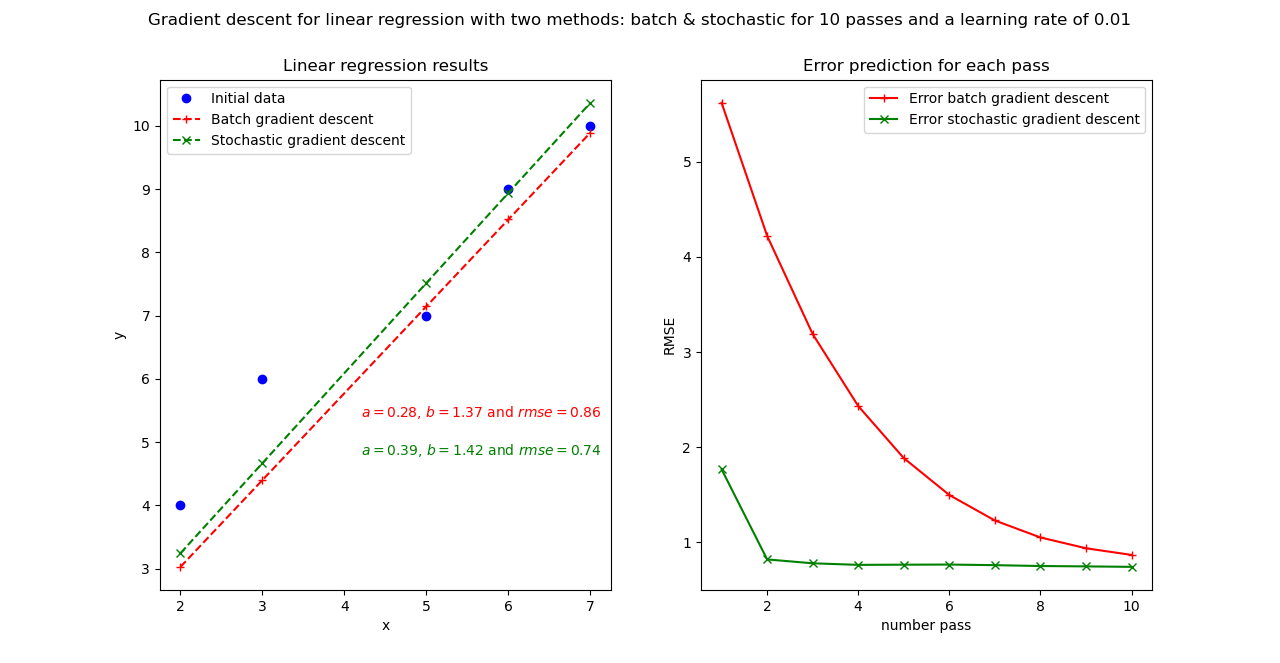
\includegraphics[width=1.05\textwidth]{Figure_GradientDescentLinearRegression.png}
\caption{Output of the tutorial in section \ref{Python tutorial}}
\end{figure}

\section{Logic details}
We show here the logic behind the gradient descent applied to a simple linear regression problem. The objective of this regression is to find the optimal slop \(b\) and intercept \(a\) which verify \(y = a + b \times x\) while minimizing the prediction error for a set of \(n\) points \((x,y)\). In this work, the error function chosen is the Sum of Squared Residuals (\(SSR\)) defined by equation (\ref{eq:1}) where \(\mathbf{v}\) is the vector of coefficients  $\begin{pmatrix}
  a \\ 
  b 
\end{pmatrix}$  and \(y_{perd}\) the predicted output variable. 

\begin{equation} \label{eq:1}
SSR(\mathbf{v}) = \frac{1}{2n}\sum_{i=1}^{n}(y_{perd}(\mathbf{v}, i)-y_{i})^{2}
\end{equation}

Using the Taylor series expansion on \(SSR(\mathbf{v})\), we obtain the equation  (\ref{eq:2}). Then, replacing \(\mathbf{\epsilon}\) by \(-\eta\nabla SSR(\mathbf{v})\) with \(\eta\) a small positive value called learning rate, we have the expression (\ref{eq:3}). 

\begin{equation} \label{eq:2}
    SSR(\mathbf{v} + \mathbf{\epsilon}) \approx SRS(\mathbf{v}) + \mathbf{\epsilon}^{T}\nabla SSR(\mathbf{v})
\end{equation}

\begin{equation} \label{eq:3}
    SSR(\mathbf{v} - \eta\nabla SSR(\mathbf{v})) \approx SSR(\mathbf{v}) - \eta\nabla SSR(\mathbf{v})^{2} \leq SSR(\mathbf{v})
\end{equation}

We deduce from the previous expression that updating \(\mathbf{v}\) by \(\mathbf{v} - \eta\nabla SSR(\mathbf{v})\) may reduce the value of \(SSR(\mathbf{v})\). This is the logic adopted by the gradient descent method consisting in the following steps: 

\begin{enumerate}
  \item Initiate the values of \(\mathbf{v}\) to zero or small random values
    \subitem [Stochastic gradient descent] Randomized the training data order giving the order array \(r\)
  \item Compute the prediction error \((y_{perd}(\mathbf{v},i)-y_{i})\) for:
        \subitem [Batch gradient descent] all training data \(\mathbf{i}\) before calculating the update
        \subitem [Stochastic gradient descent] each training data instance \(\mathbf{i}\) and calculate the update immediately
  \item Compute the update of \(\mathbf{v}\) with: 
      \subitem [Batch gradient descent] \(i\subset[1,n]\)
        \begin{equation} \label{eq:4}
            \begin{cases}
            a := a - \eta\frac{\partial SSR(\mathbf{v}, i)}{\partial a} = a - \frac{\eta}{n}\sum_{i=1}^{n}(y_{perd}(\mathbf{v}, i)-y_{i})\\
            b := b - \eta\frac{\partial SSR(\mathbf{v}, i)}{\partial b} = b - \frac{\eta}{n}\sum_{i=1}^{n}(y_{perd}(\mathbf{v}, i)-y_{i})x_{i}
            \end{cases}
        \end{equation}
      \subitem [Stochastic gradient descent] \(i = r[j]\) with j the iteration of the gradient descent 
          \begin{equation} \label{eq:5}
            \begin{cases}
            a := a - \eta\frac{\partial SSR(\mathbf{v}, r[j])}{\partial a} = a - \eta(y_{perd}(\mathbf{v}, r[j])-y_{r[j]})\\
            b := b - \eta\frac{\partial SSR(\mathbf{v}, r[j])}{\partial b} = b - \eta(y_{perd}(\mathbf{v}, r[j])-y_{r[j]})x_{r[j]}
            \end{cases}
          \end{equation}
  \item Repeat the steps 2 and 3 until reaching "good" enough coefficients. The performance threshold \(th_{p}\) could be defined as value on the Root Mean Square Error (\(RMSE\)) such that we should verify:
    \begin{equation}
          RMSE = \sqrt{\frac{\sum_{i=0}^{n}(y_{i}^{pred} - y_{i})^{2}}{n}} < th_{p}
    \end{equation}
\end{enumerate}

Remarks: the stochastic gradient descent is preferred to the batch one for large datasets. To note also that stochastic gradient descent will require a small number of passes through the dataset to reach "good" enough coefficients typically between 1-to-10 passes. 

\newpage
\section{Python tutorial} \label{Python tutorial}
The code source displayed below can be found on \href{https://github.com/SophMarch/Tutorials}{GitHub} under Python\_GradientDescentLinearRegression.py
\lstinputlisting[language=Python]{Python_GradientDescentLinearRegression.py}

\end{document}
